\chapter{Android}
\label{ch:Android}
Android is a mobile operating system developed by Google, based on the Linux kernel. Android's primary focus is on mobile handheld devices with a touchscreen. The most popular examples would be smartphones, tablets and everything in between, like phablets. Android is open source which means developers can modify the underlying operating system as they wish. Android programs are called ``apps'' which is the short version of application, these applications extend the basic functionality of an Android device.

\section{History of Android}
Android started as a startup Company under the name ``Android Inc.'' It was founded in Palo Alto, California in October 2003. It was meant to be an advanced operating system for digital cameras. In 2004 they changed their goals to expand their operating system to handheld devices that can compete against Symbian and other mobile operating systems which were state of the art at this time. In July 2005 Google bought the whole company along with its key employees for a huge amount of money, 50 Million U.S. dollar at least, according to rumors. They developed a prototype which had similarities with a BlackBerry phone, it had no touchscreen and a physical QWERTY keyboard. Due to the launch of the Apple iPhone in 2007, Google changed its Android specification documents to state that "Touchscreens will be supported", although "the Product was designed with the presence of discrete physical buttons as an assumption, therefore a touchscreen cannot completely replace physical buttons". The first commercially available smartphone using Android as its operating system was the HTC Dream announced in 2008. Since then Google launched numerous updates which improved the operating system bit by bit. They fixed bugs from prior releases and added new features along the way. Android major versions also have a naming scheme, they are all named after a dessert or a sugary treat. Each version starting with the next character in the alphabet starting with version 1.5 called ``Cupcake'', followed by 1.6 as ``Donut'' up to 7.0 as ``Nougat'' and the current version 8.0 as ``Oreo''. Google explained this naming scheme with the following sentence ``Since these devices make our lives so sweet, each Android version is named after a dessert''.

\section{Overview of Android Application Development}
 Applications are often abbreviated as ``apps''. These Android apps are written using the Android software development kit (SDK). There are a small selection of programming languages available that can be used to develop a native Android app.

\subsection{Java}
Java is the most popular language to develop an Android application. The majority of apps and libraries are written in Java. These apps are compiled to bytecode for the Java virtual machine, which is then translated to Dalvik bytecode. The Dalvik virtual machine is a process virtual machine developed for the Android platform. Since Android 5.0 Dalvik is discontinued and the Android Runtime was introduced, which now translates the application's bytecode into native instructions.

\subsection{C/C++}
With C or C++ Code and the Android native development kit (NDK), a native library for Android, applications can get much better results in terms of performance. Because the C or C++ Code runs natively on the device it executes faster than the Java code run in the Android runtime environment. The only downside of this is that all of the C or C++ code needs to be handled through the Java native interface (JNI). This programming framework handles the interoperability of the Java code and the C/C++ Code.

\subsection{Go}
The Go programming language is an open source project developed by a team at Google and many contributers from the open source community \cite{GoProject}. This programming language is supported although there are limitations to the application programming interfaces (API).

\subsection{Kotlin}
In May 2017, Google announced official support for the Kotlin Programming language. Kotlin is a modern and powerful language and solved some issues addressed with Java (e.g. Null references). Kotlin is also interoperable with Java which means Kotlin can be used in already existing Java projects.

\section{Design}
Material Design is Google's visual design language that was first introduced in 2014. The goal was to develop a single underlying system that allows for a unified experience across all kinds of devices. It tries to support visual elements with the characteristics of real materials, hence Material Design. These guidelines help the users to interact and quickly understand different kinds of User Interface (UI) elements by using familiar tactile attributes.

GRAMOC's Android app uses these design principles for the user interface as shown in figure \ref{fig:appscreenshots}

\begin{figure}[H]
	\centering
	\begin{tabular}{cc}
	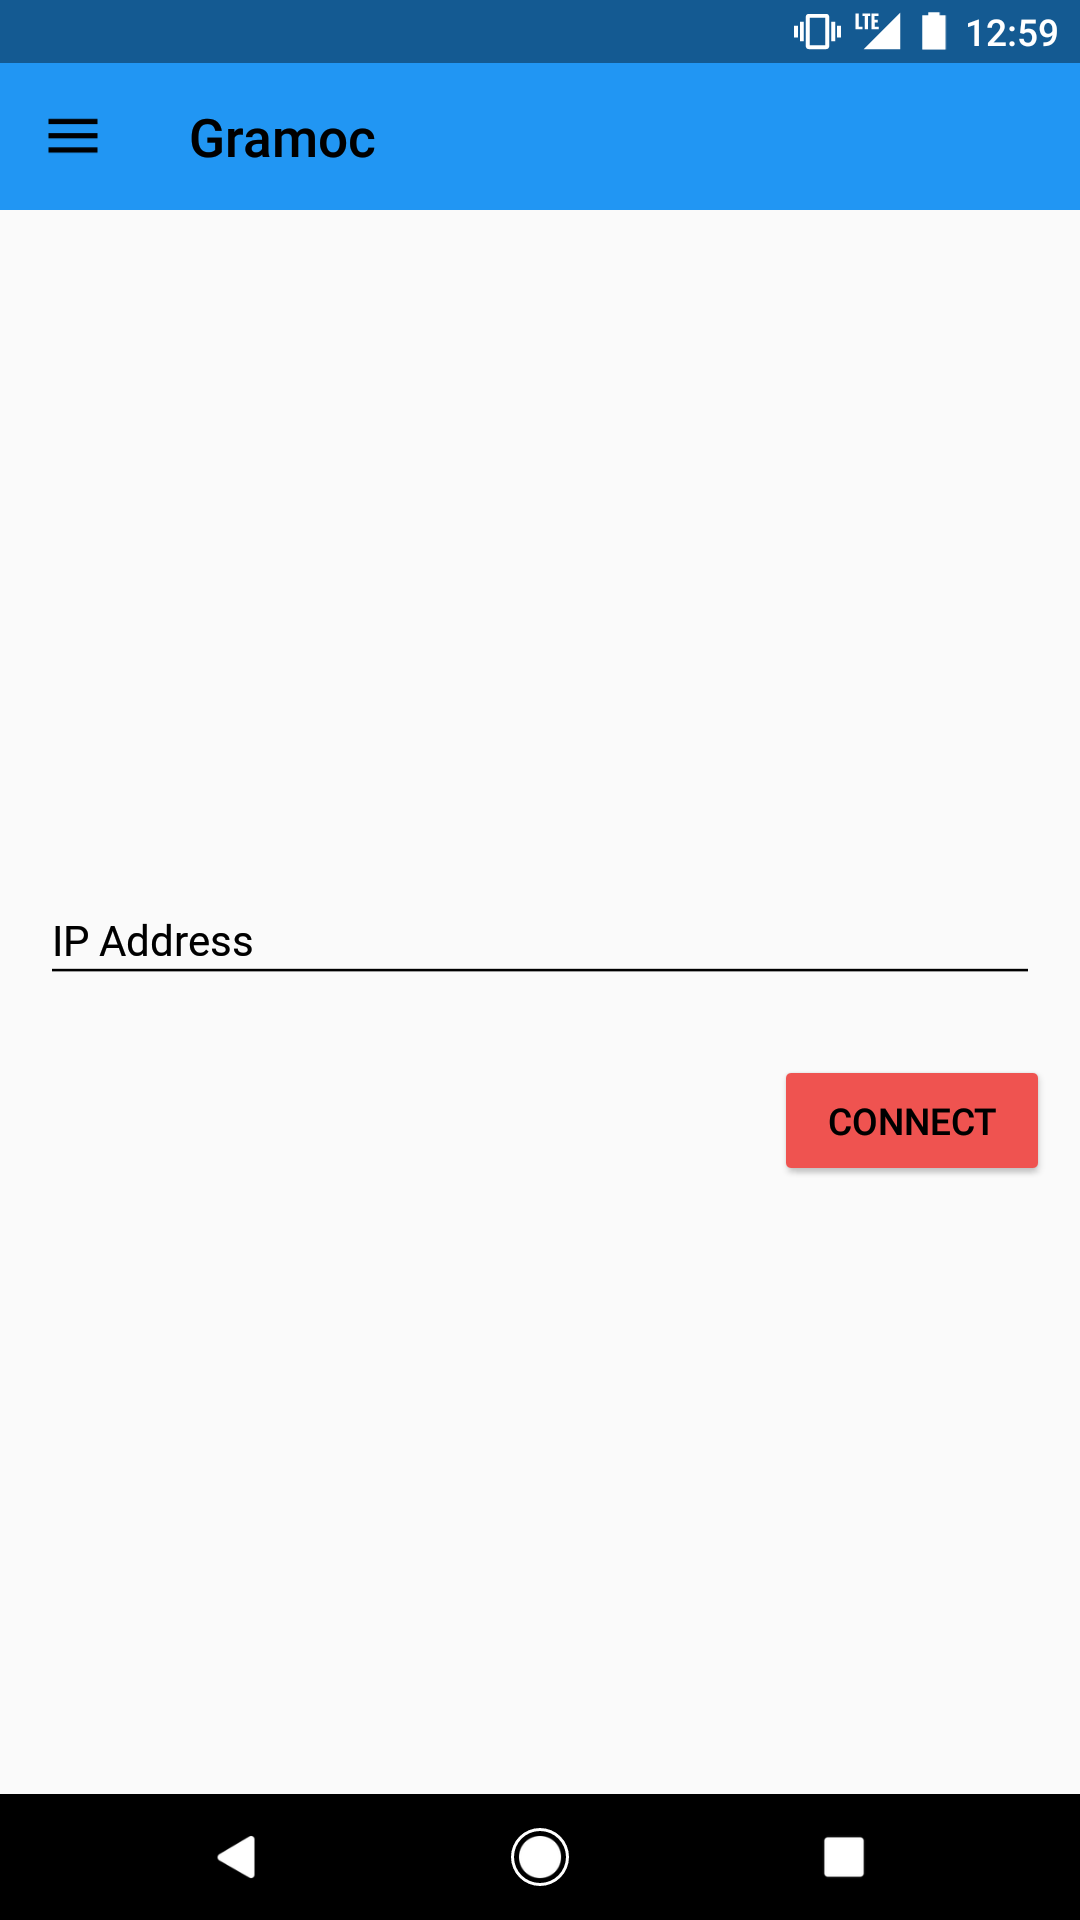
\includegraphics[height=7cm,keepaspectratio]{app_connect}
	&
	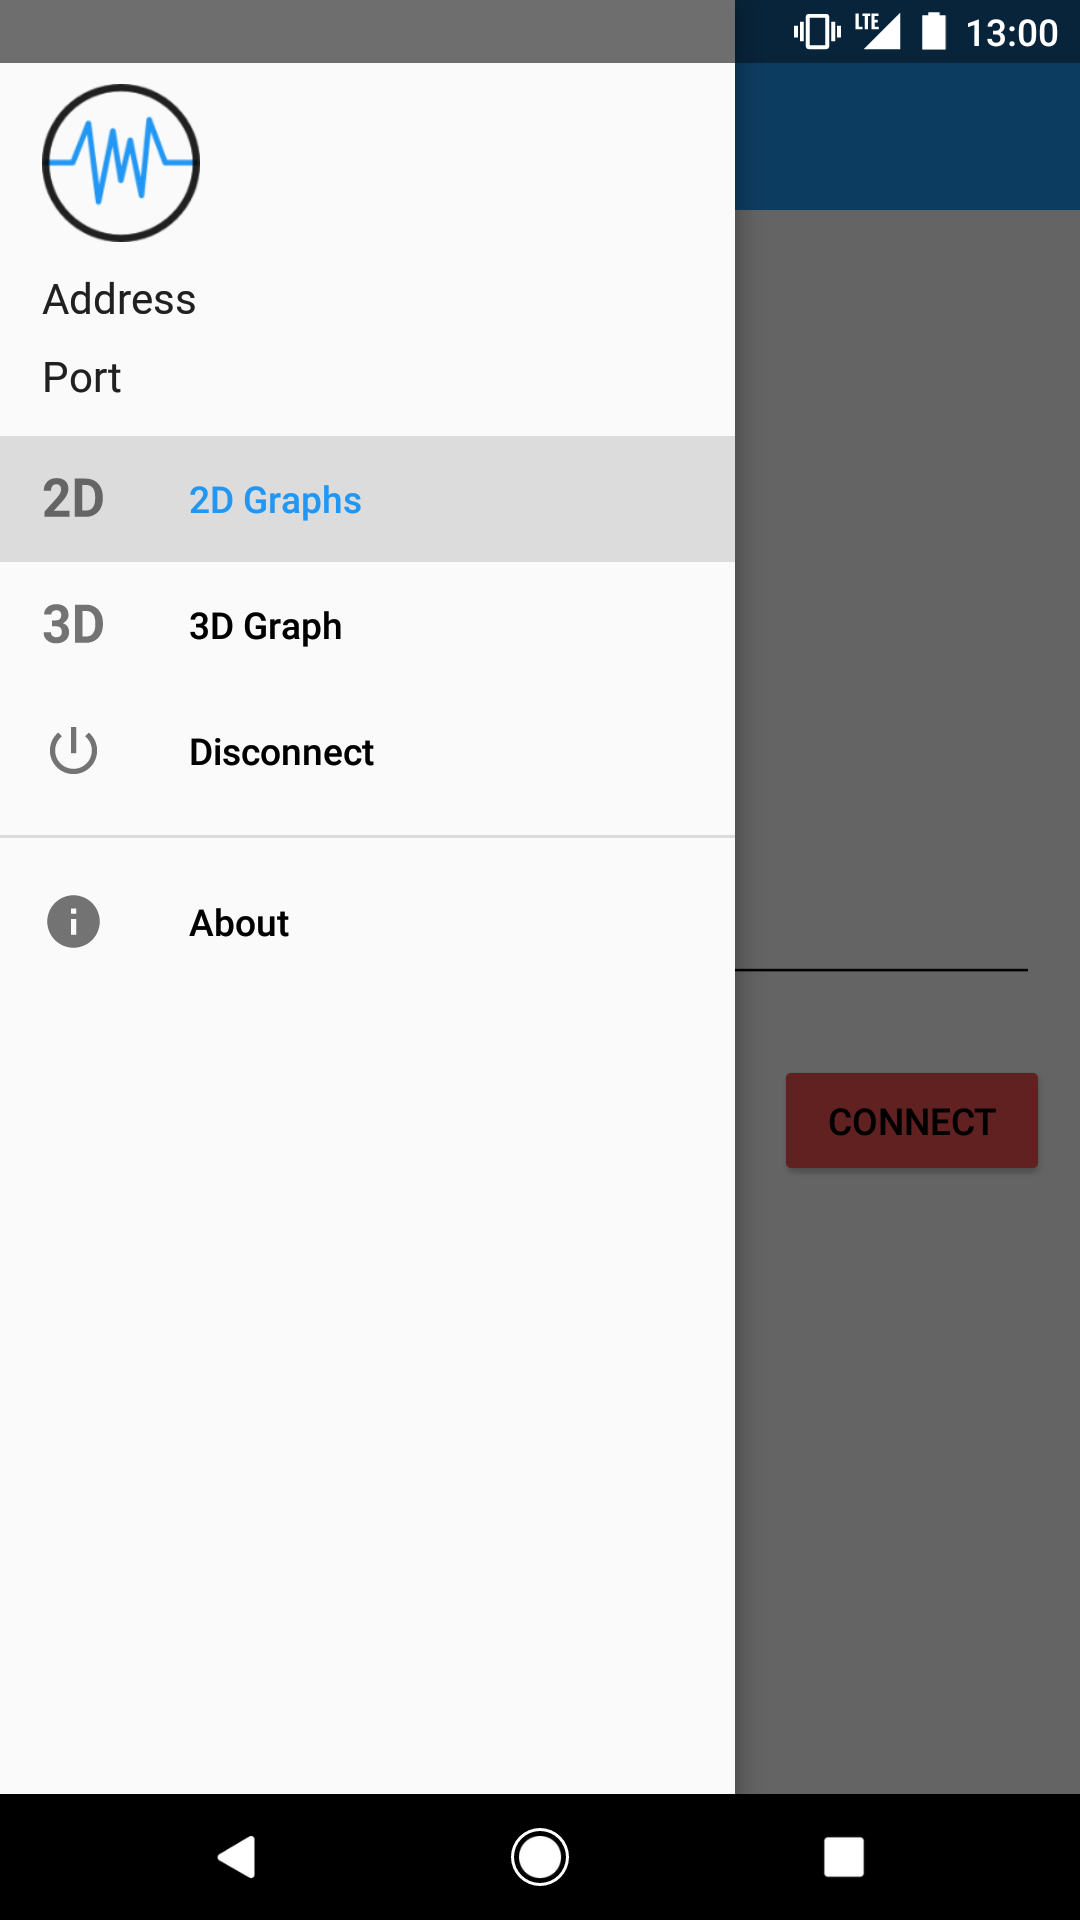
\includegraphics[height=7cm,keepaspectratio]{app_navdrawer}
	\\
	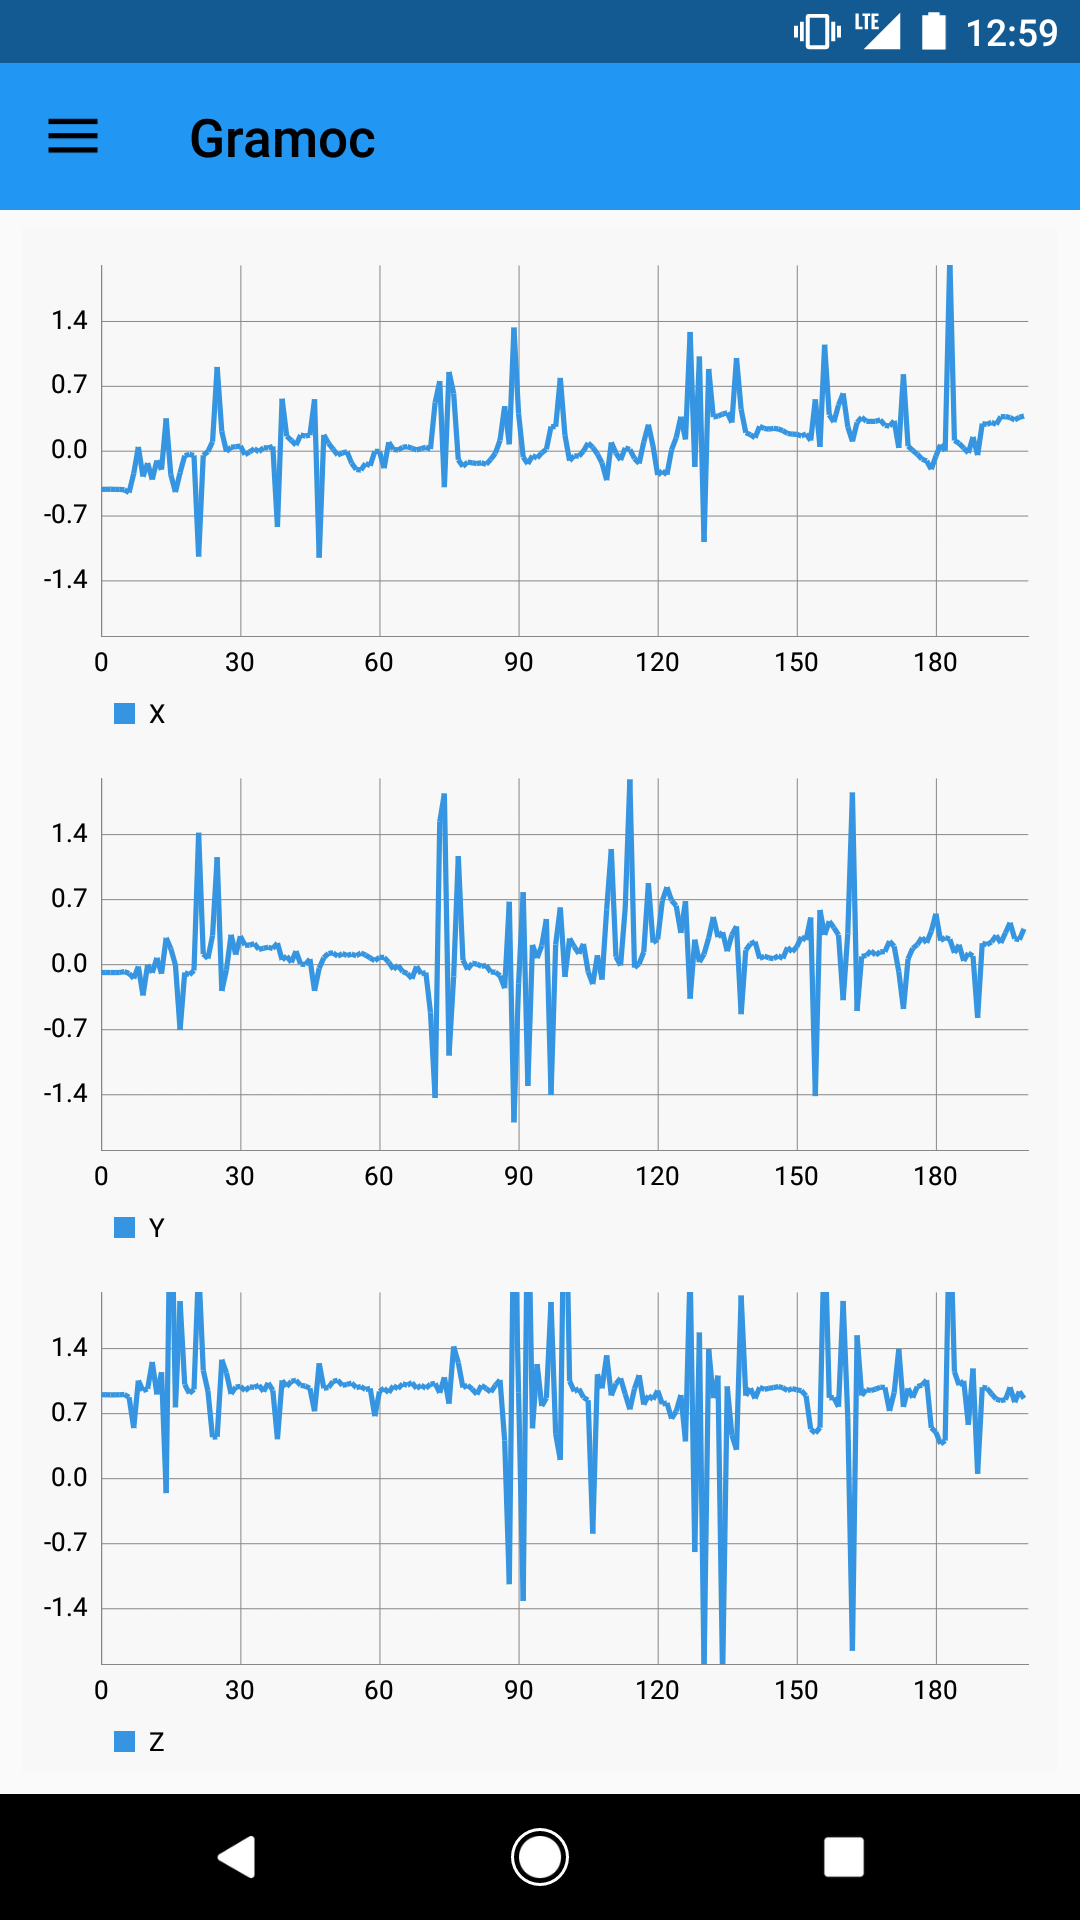
\includegraphics[height=7cm,keepaspectratio]{app_sensor}
	&
	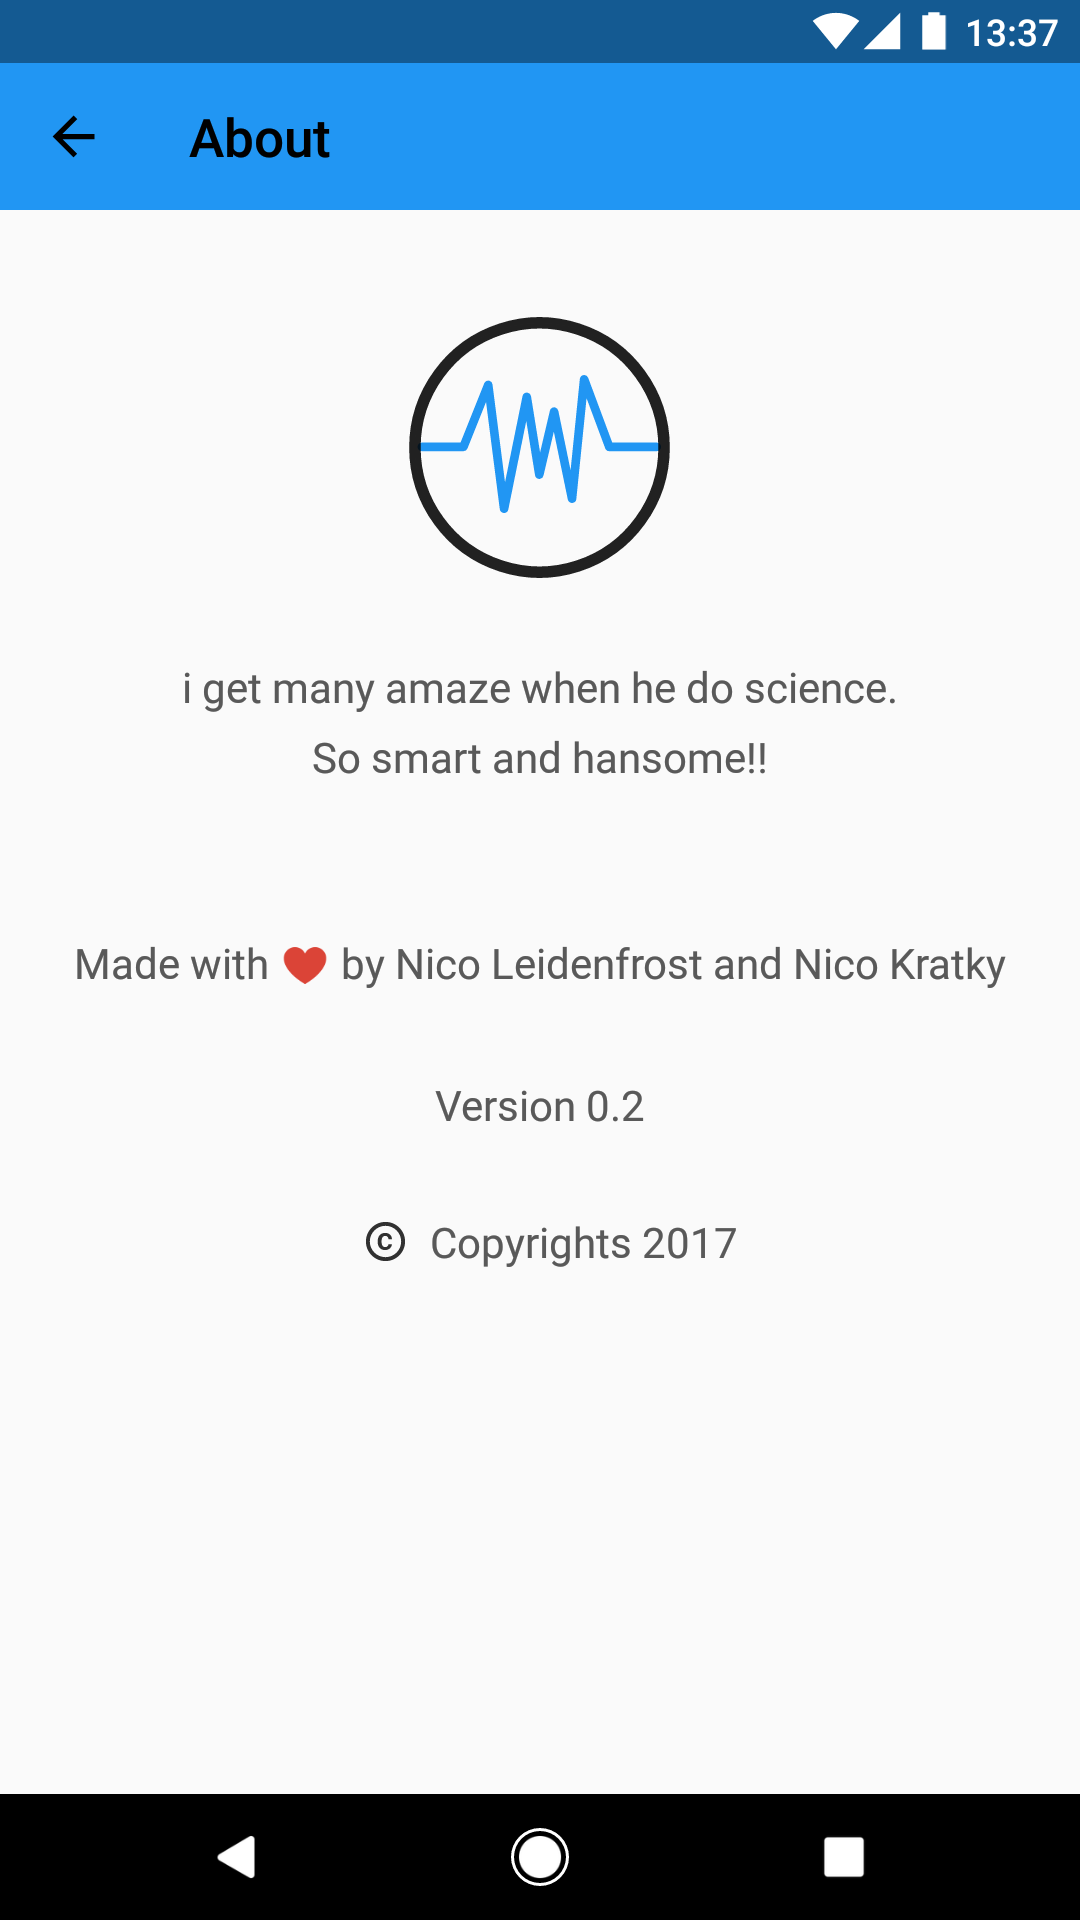
\includegraphics[height=7cm,keepaspectratio]{app_about}
	\end{tabular}
	\caption{Screenshots of App}
	\label{fig:appscreenshots}
\end{figure}

\section{Components}
In order to build this Android application following Android components were used:

\begin{itemize}
	\item Intent
	\item Toolbar
	\item Activity
	\item Service
	\item NavigationDrawer
	\item Threads
\end{itemize}

\subsection{Intent}
An intent is an abstract description of an operation to be performed \cite{AndroidIntent}. It takes an action that has to be performed and data to operate on and handles the execution of this particular action. It's most used when launching a new activity.

\subsection{Toolbar}
This component is a widget from the Android \emph{appcompat support library} and is usually used as an app bar, also known as the action bar. The most important functions of such a bar is to make space for identification of an application and to create an easy way to perform important actions, like search or navigation.

\subsection{Activity}
``An activity is a single, focused thing that the user can do.'' \cite{AndroidActivity} An activity is the main entry point of an application, it takes care of creating a new window and loading all the User Interface (UI) elements. Activities are usually shown as a full-screen window, but they can also be used as a floating window or even be embedded inside of another activity by implementing an ActivityGroup. Inside the Android-system, activities are managed as a stack, this means when a new activity is started it will be placed on top of this stack and become the running activity, the other activities are placed below this one in the stack and therefore remain inactive. The lifecycle of such an activity can be described as in Figure \ref{fig:activitylifecycle}.

\begin{figure}[H]
	\centering
	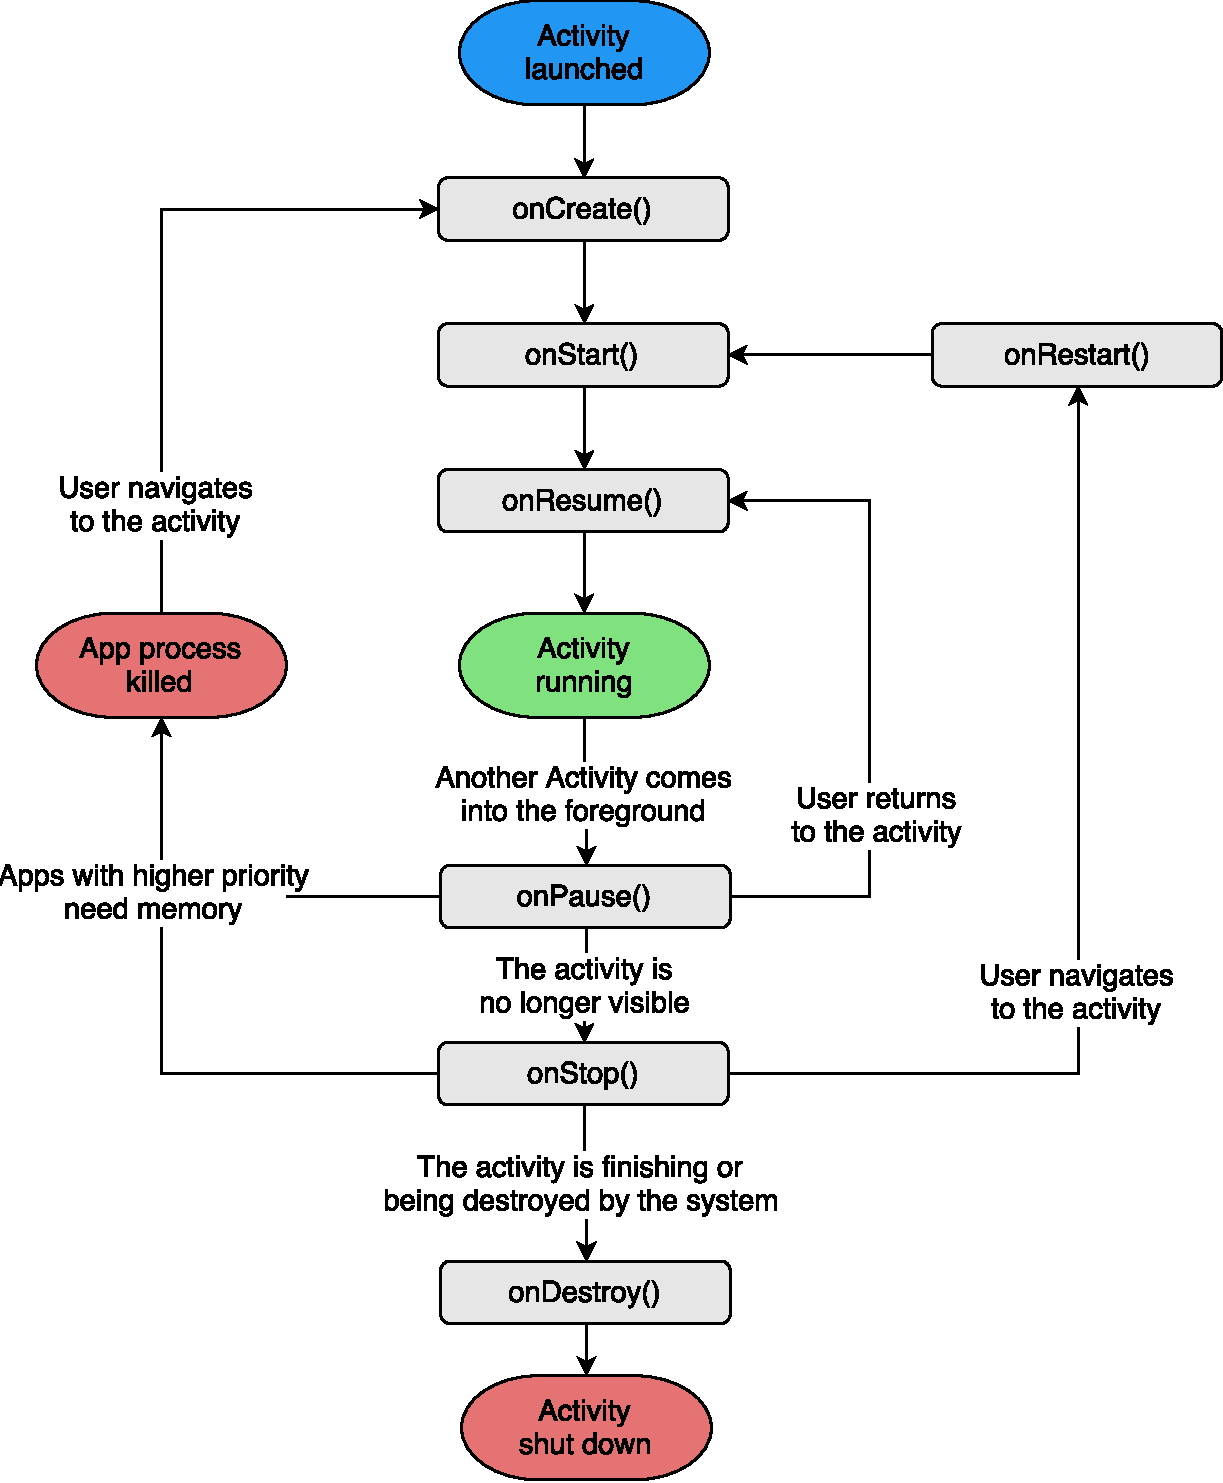
\includegraphics[width=10cm,keepaspectratio]{android-activity-lifecycle}
	\caption{Flowchart showing the lifecycle of an Android-activity}
	\label{fig:activitylifecycle}
\end{figure}

\subsection{Service}
A service is used to perform long-running operations in the background, because it's there it does not need a user interface like an activity. Once started a service can persist even if the user switches to another application. If another component binds itself to the service, it enables the possibility of interprocess communication (IPC). A typical example for a service is to handle network connections through it. The lifecycle is described as in Figure \ref{fig:servicelifecycle}.

\begin{figure}[H]
	\centering
	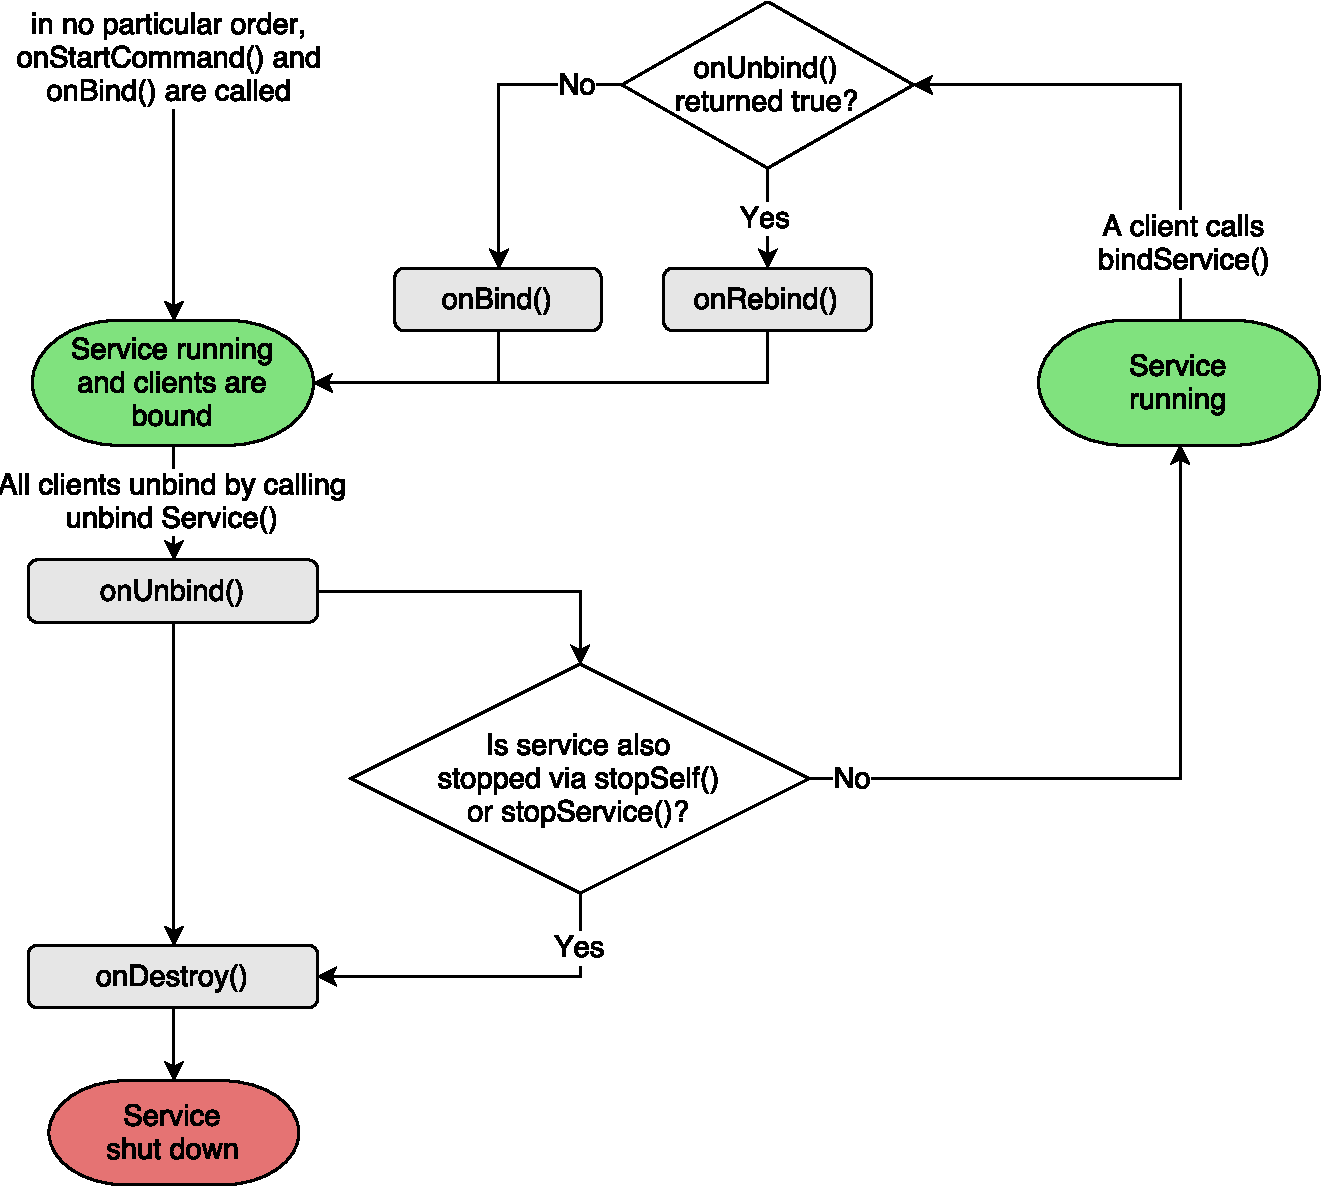
\includegraphics[width=10cm,keepaspectratio]{android-service-lifecycle}
	\caption{Flowchart showing the lifecycle of an Android-service}
	\label{fig:servicelifecycle}
\end{figure}

\subsection{NavigationDrawer}
To navigate to the different activities and views a navigation drawer was implemented. In other words this is a panel that swipes in from the left side of the screen to approximately 3 quarters of the screen width and consists of a header where general information is displayed and a body which is filled with different navigation items. A navigation drawer is part of the material design patterns and therefore commonly used in applications which implement this kind of design.

\subsection{Threads}
When an Android application component starts and no other component of the same application is already started Android will start a new Linux process. On the other hand if an application component is started and there is already a process of this application running, Android will launch the component in the main-thread of this application unless it's explicitly started in a new thread within this process. There are two essential rules to follow when dealing with threads in Android:

\begin{enumerate}
	\item Do not block the UI Thread
	\item Do not access the Android UI toolkit from outside the UI thread
\end{enumerate}

\noindent There are a few different ways how to execute tasks asynchronous in Android:

	\subsubsection{Extended Threads}
	The first possible solution is to create a subclass of the Java \emph{Thread} class. If this method is chosen the \emph{run} method of the superclass Thread needs to be overwritten. This method is recommended if the behavior of the threads needs to be modified or new functionalities needs to be implemented, otherwise implementing the Runnable interface would be more appropriate.

	\subsubsection{Runnable interface}
	Another way to accomplish asynchronous behavior is to create a class that implements the \emph{Runnable} interface. An Instance of this class can then be passed to the specific thread in which the tasks are executed. This method is preferred to use when running tasks without the need of modified thread behavior because a runnable class won't need to create a new thread every time it executes. Also a runnable class can be executed on different threads.

	\subsubsection{AsyncTasks}
	AsyncTasks are used to do work in the background and then update the UI accordingly. As AsyncTasks are defined to do blocking operations there can be only one running AsyncTask at a time. There are four steps that will be executed when performing an AsyncTask:

	\begin{enumerate}
		\item \textbf{onPreExecute}: executed on the UI thread before the task is executed.
		\item \textbf{doInBackground}: executed on the background thread, here the background work that needs to be done is executed.
		\item \textbf{onProgressUpdate}: executed on the UI thread every time when \emph{publishProgress} is called in the background thread.
		\item \textbf{onPostExecute}: executed on the UI thread when the background tasks are finished.
	\end{enumerate}

\subsection{Libraries}
The Android client was implemented using a small number of libraries:
\begin{itemize}
	\item \textbf{Android SDK}

	The standard libraries included in the Android platform itself \cite{AndroidSDK}.

	\item \textbf{GramocAlgorithm-client}

	The Java implementation of the GSDEP client developed along with this project \cite{GramocAlgorithm-client}.

	\item \textbf{MPAndroidChart}

	An easy to use but also powerful open source 2 dimensional chart library for Android \cite{MPAndroidChart}.

	\item \textbf{android-about-page}

	This library allows to simply create an about page for your Android application \cite{android-about-page}.
\end{itemize}

\section{Implementation}
The entry point of this Android application is called the \emph{MainActivity}. When this Activity starts a background service is also started which is basically a wrapper for the GSDEP client, therefore it handles all the networking related tasks within the app. The service will be bound to the active activity, so every time another activity is launched the service will be unbound by the current activity and newly bound by the starting activity. The \emph{MainActivity's} goal is to give the user an easy way to connect to the server. Once the application successfully connects to the server, a new activity responsible for plotting the received sensor data will be launched, whether the 2 dimensional or the 3 dimensional plotting activity is launched depends on the selection made in the \emph{NavigationDrawer}, by default the 2 dimensional plotting activity will be launched. {\color{red} \textbf{(MAYBE REMOVE 3D ACTIVITY?)}} When the 2 dimensional plotting activity is launched the networking service will be bound and three \emph{LineCharts} contained within the library \emph{MPAndroidChart} will be created and properly set up. After these tasks are finished and the activity is ready to receive data the server will be notified. Now each data set received will be added to the data buffer of the respective chart. If the buffer of a chart is full, the values at the end will be truncated until there is enough space to add the new values.
